\documentclass[aps,pra,twocolumn,reprint,amsmath,amssymb,floatfix]{revtex4-2}

\usepackage{graphicx}
\usepackage{booktabs}
\usepackage{siunitx}
\usepackage[colorlinks=true,linkcolor=blue,citecolor=blue,urlcolor=blue]{hyperref}
\usepackage{float}
\usepackage{xcolor}
\usepackage{array}
\usepackage{tabularx}
\usepackage{braket}

\begin{document}

\title{Holographic Cluster-State Synthesis in Circuit QED:\\
Corrected Exclusive-Family Reanalysis}

\author{Autonomous Research Agent}
\affiliation{Quantum Circuits Group}
\date{\today}

\begin{abstract}
We revisit the corrected exclusive-family holographic cluster-state study for a
dispersive transmon-cavity platform and extend it in two directions. The
baseline branch keeps the full logical target
$\mathrm{SWAP}\cdot\mathrm{CZ}\cdot(H\otimes I)$ on
$\{\ket{g,0},\ket{g,1},\ket{e,0},\ket{e,1}\}$ and performs the completed
exclusive-family design-space search over $D+R+\mathrm{SQR}$ and
$D+R+\mathrm{CPSQR}$. The follow-up branch then replaces that target with the
restricted ground-sector transfer
$U_{\mathrm{joint}}(\ket{g}\otimes\ket{\psi})\approx
\ket{g}\otimes H_c\ket{\psi}$ on $\{\ket{g,0},\ket{g,1}\}$, where $H_c$ is
the logical cavity Hadamard. We retain the 216-point structural screen, 30
level-subset refinements, and 12 physical full-target finalists as the
baseline, then re-score one representative per family and block count under the
reduced objective and run a targeted local restricted-target refinement at
$N_{\mathrm{cav}}=12$ with validation at $N_{\mathrm{cav}}=10,12,14$.

The full-target branch confirms the earlier corrected conclusion that both
exclusive families can exceed $99\%$ in the closed-system ideal-unitary metric,
with the best SQR solution reaching $F_{12}=0.9996347$ and the best CPSQR
solution reaching $F_{12}=0.9974917$. However, those same winners are poor
ground-sector transfers: when rescored under the reduced objective, their
restricted fidelities collapse to about $0.50$ because they excite the ancilla
almost completely. After local restricted-target refinement, both families
cross $0.99$ already at three blocks. The best absolute reduced-objective
solutions are a 5-block SQR $RDS$ sequence with
$F_{\mathrm{ground},12}=0.9999260$ and a 4-block CPSQR $RDCP$ sequence with
$F_{\mathrm{ground},12}=0.9999284$, both with outside-target leakage below
$2\times10^{-4}$. Two-block representatives remain just below threshold. The
reduced objective therefore changes both the minimum-depth answer and the family
ranking relative to the full-target problem. Direct GRAPE remains a separate
full-target reference with open-system validation, but its best replay point is
still only $0.9760$ at \SI{800}{ns}. Open-system validation of the new
ground-sector winners remains future work.
\end{abstract}

\maketitle

\section{Introduction}

Holographic generation of one-dimensional cluster states uses a repeated
per-site transfer unitary to build entanglement bond by bond with a small
physical register \cite{raussendorf2001one,briegel2001persistent}.
In circuit QED this register is naturally realized by a transmon dispersively
coupled to a long-lived cavity mode, where the transmon carries the fresh site
and the cavity stores the bond history \cite{blais2021circuit,ofek2016extending}.

The previous unified study consolidated several exploratory decomposition and
validation passes, but it also mixed gate families that are not part of the
corrected user scope. This report therefore rewrites the study around two
exclusive structured families only:
\begin{enumerate}
  \item $D + R + \mathrm{SQR}$,
  \item $D + R + \mathrm{CPSQR}$.
\end{enumerate}
Direct GRAPE is retained only as an external reference point for speed and
validated pulse performance, not as part of the structured-family comparison.

This report now adds a second layer on top of that corrected full-target study.
The baseline search answers the original joint logical task. The follow-up asks
whether the same structured families can implement the weaker but physically
important reduced map
$U_{\mathrm{joint}}(\ket{g}\otimes\ket{\psi})\approx
\ket{g}\otimes H_c\ket{\psi}$ on the ground ancilla sector, and whether that
reduced objective changes the depth ranking or family preference. As shown
below, it does: the full-target winners are not reusable as ground-sector
solutions, and the restricted objective becomes a genuinely different control
problem rather than a mild relaxation of the original one.

The second correction is methodological: results at
$N_{\mathrm{cav}}\leq 8$ are treated as preliminary only. Final evidence must
come from $N_{\mathrm{cav}}>8$, with $N_{\mathrm{cav}}=12$ as the default final
truncation and additional checks at $N_{\mathrm{cav}}=10,14$. The third
correction is an explicit active-subspace rule based on sampled cavity
population during the full evolution. These three changes are enough to alter
the structured-family ranking.

\section{System and Methods}

\subsection{Target and Hamiltonian}

The logical basis is
\begin{equation}
\mathcal{B}_{\mathrm{log}} =
\{\ket{g,0},\ket{g,1},\ket{e,0},\ket{e,1}\},
\end{equation}
and the target unitary is
\begin{equation}
U_{\mathrm{target}} = \mathrm{SWAP}\cdot\mathrm{CZ}\cdot(H\otimes I).
\end{equation}
All structured optimizations use the dispersive transmon-cavity Hamiltonian
\cite{blais2021circuit}
\begin{align}
\hat{H}/\hbar &= \omega_c a^\dagger a + \omega_q b^\dagger b
+ \frac{\alpha}{2}b^\dagger b(b^\dagger b-1) \notag \\
&\quad + \chi a^\dagger a\,b^\dagger b
+ \chi' a^{\dagger 2} a^2 b^\dagger b + K a^{\dagger 2} a^2.
\end{align}

\begin{table}[htbp]
\centering
\caption{Physical parameters used throughout the corrected study.}
\label{tab:params}
\begin{tabular}{@{}lll@{}}
\toprule
Parameter & Value & Unit \\
\midrule
$\omega_c/2\pi$ & 5.241 & GHz \\
$\omega_q/2\pi$ & 6.150 & GHz \\
$\alpha/2\pi$   & -255 & MHz \\
$\chi/2\pi$     & -2.84 & MHz \\
$\chi'/2\pi$    & -21 & kHz \\
$K/2\pi$        & -28 & kHz \\
$N_{\mathrm{tr}}$ & 2 & levels \\
\bottomrule
\end{tabular}
\end{table}

\subsection{Corrected family scope}

Only two structured families are studied:
\begin{itemize}
  \item $D+R+\mathrm{SQR}$ with two through five selective blocks,
  \item $D+R+\mathrm{CPSQR}$ with one through five conditional-phase blocks.
\end{itemize}
No mixed SQR/CPSQR family appears in the search, tables, ranking, discussion,
or conclusions.

The finalized design-space search is implemented in
\texttt{scripts/run\_design\_space\_study.py}. The screen covers all six
orderings of the three gate types, active-tone budgets
$n_{\mathrm{active}}\in\{1,2,3,4\}$, and the block ranges listed above, for a
total of 216 structural cases at $N_{\mathrm{cav}}=4$. The strongest
structures are then refined over level subsets at the same truncation, and the
best 12 finalists are re-optimized directly at $N_{\mathrm{cav}}=12$ before
being validated at $N_{\mathrm{cav}}=10,12,14$.

\subsection{Active-subspace rule}

For each candidate and each logical input, the full gate sequence is sampled
gate-by-gate with intermediate fractional steps. The active cavity subspace is
defined by the following rule:
\begin{enumerate}
  \item include all Fock levels whose peak population is at least $10^{-3}$,
  \item expand this set until the worst instantaneous captured population is at
  least $99.9\%$.
\end{enumerate}
We report both per-input active levels and the candidate-wide union. A
candidate is flagged as low confidence or discarded if its active support runs
to the truncation boundary or if the worst logical leakage remains large.

\subsection{Retention criteria}

The corrected study uses $N_{\mathrm{cav}}=12$ as the default final evidence
and checks consistency at $N_{\mathrm{cav}}=10,14$. In practice, three signals
drive the decision:
\begin{itemize}
  \item fidelity at $N_{\mathrm{cav}}=12$,
  \item worst logical leakage at $N_{\mathrm{cav}}=12$,
  \item whether the active cavity support touches the truncation boundary.
\end{itemize}
Under these rules, a candidate can be retained as low confidence if its
fidelity is stable and its support is bounded but its leakage remains above the
stricter comfort threshold.

\subsection{Ground-sector follow-up metric}

For the follow-up branch we restrict attention to the subspace
\begin{equation}
\mathcal{G} = \{\ket{g,0},\ket{g,1}\},
\end{equation}
and define the cavity-only target
\begin{equation}
H_c = \frac{1}{\sqrt{2}}
\begin{pmatrix}
1 & 1 \\
1 & -1
\end{pmatrix}.
\end{equation}
If $U$ is the full closed-system sequence unitary and $P_g$ projects onto
\(\mathcal{G}\), then the reduced target comparison uses the restricted block
\begin{equation}
U_{gg} = P_g U P_g
\end{equation}
and the process-fidelity measure
\begin{equation}
F_{\mathrm{ground}} = \frac{|\mathrm{Tr}(H_c^{\dagger} U_{gg})|^2}{4}.
\end{equation}
We also split leakage from ground-sector inputs into two components: ancilla
excitation, meaning population transferred to \(\ket{e,n}\), and cavity-support
spillover inside the ground manifold but outside \(\{\ket{g,0},\ket{g,1}\}\).
The restricted-target follow-up re-scores the best saved full-target
representative for each family and block count, then warm-starts one local
restricted-target refinement per block representative at
\(N_{\mathrm{cav}}=12\) and re-checks the refined solutions at
\(N_{\mathrm{cav}}=10,12,14\).

\section{Results}

\subsection{Preliminary search results}

Table~\ref{tab:prelim} shows the best coarse-screen candidate from each
exclusive family at $N_{\mathrm{cav}}=4$. The search already indicates two key
features of the landscape. First, both families benefit strongly from deeper
circuits: the strongest preliminary candidates sit at five blocks. Second, the
best SQR screen point already prefers the $RDS$ ordering with the full
four-tone budget, whereas the best CPSQR screen point is still a four-tone
solution and has not yet identified the leaner two-tone finalist that emerges
after the targeted $N_{\mathrm{cav}}=12$ refinement.

\begin{table*}[t]
\centering
\caption{Best preliminary candidate from each exclusive family at
$N_{\mathrm{cav}}=4$, after the full structural screen and finalist replay at
$N_{\mathrm{cav}}=12$.}
\label{tab:prelim}
\begin{tabular}{@{}lccccccc@{}}
\toprule
Family & Blocks & $n_{\mathrm{active}}$ & Order & Levels & Ideal $F_4$ & Replay $F_{12}$ & Time (ns) \\
\midrule
$D+R+\mathrm{SQR}$ & 5 & 4 & RDS & $\{0,1,2,3\}$ & 0.99929 & 0.99430 & 6180 \\
$D+R+\mathrm{CPSQR}$ & 5 & 4 & DCPR & $\{0,1,2,3\}$ & 0.99851 & 0.98976 & 1445 \\
\bottomrule
\end{tabular}
\end{table*}

The coarse screen already places both families close to the $99\%$ target, but
their tradeoffs differ sharply. The SQR family pushes fidelity upward by using
all four tones and the deepest sequence in the study. The CPSQR family reaches
almost the same preliminary fidelity with a much shorter sequence, but its best
coarse-screen point still carries leakage slightly above the stricter
retention threshold. Those differences motivate the targeted finalist
refinement.

\subsection{Design-space trends}

Figure~\ref{fig:heatmaps} and Fig.~\ref{fig:ordering} summarize the screened
design landscape. In both exclusive families the dominant factor is block
count. For SQR the best coarse-screen replay fidelity rises from 0.627 for two
blocks to 0.704 for four blocks, with a smaller but still visible improvement
from increasing the active-tone budget from one tone to four. For CPSQR the
depth effect is much stronger: the best replay fidelity climbs from 0.500 at
one block to 0.931 at four blocks, far larger than the effects of either
ordering or tone budget. This identifies circuit depth as the most important
resource knob in both families.

Ordering is the second major lever, but it behaves differently in the two
families. For SQR the three strongest orderings in the screen are clustered
closely: DSR has the best median replay performance, with DRS and RDS nearly
degenerate. For CPSQR the spread is wider. CPDR has the best median replay
score, while RDCP and DRCP produce the strongest individual screen points.
That separation between median robustness and best-case performance turns out
to matter in the finalist stage.

A dedicated fixed-budget re-optimization of the shortlisted SQR orderings
resolves that near-degeneracy in favor of $RDS$. At a common local budget
($\texttt{maxiter}=24$), $RDS$ reaches $F_{12}=0.998389$ with worst leakage
$4.86\times 10^{-3}$, followed by $DSR$ at $0.998064$ and $SDR$ at $0.997194$,
while the original $DRS$ order falls to $0.992561$ with worst leakage
$2.50\times10^{-2}$. The earlier impression that $DRS$ should be treated as
effectively tied with the leading SQR orders is therefore not supported once
the finalists are compared under a common refinement budget.

\begin{figure*}[t]
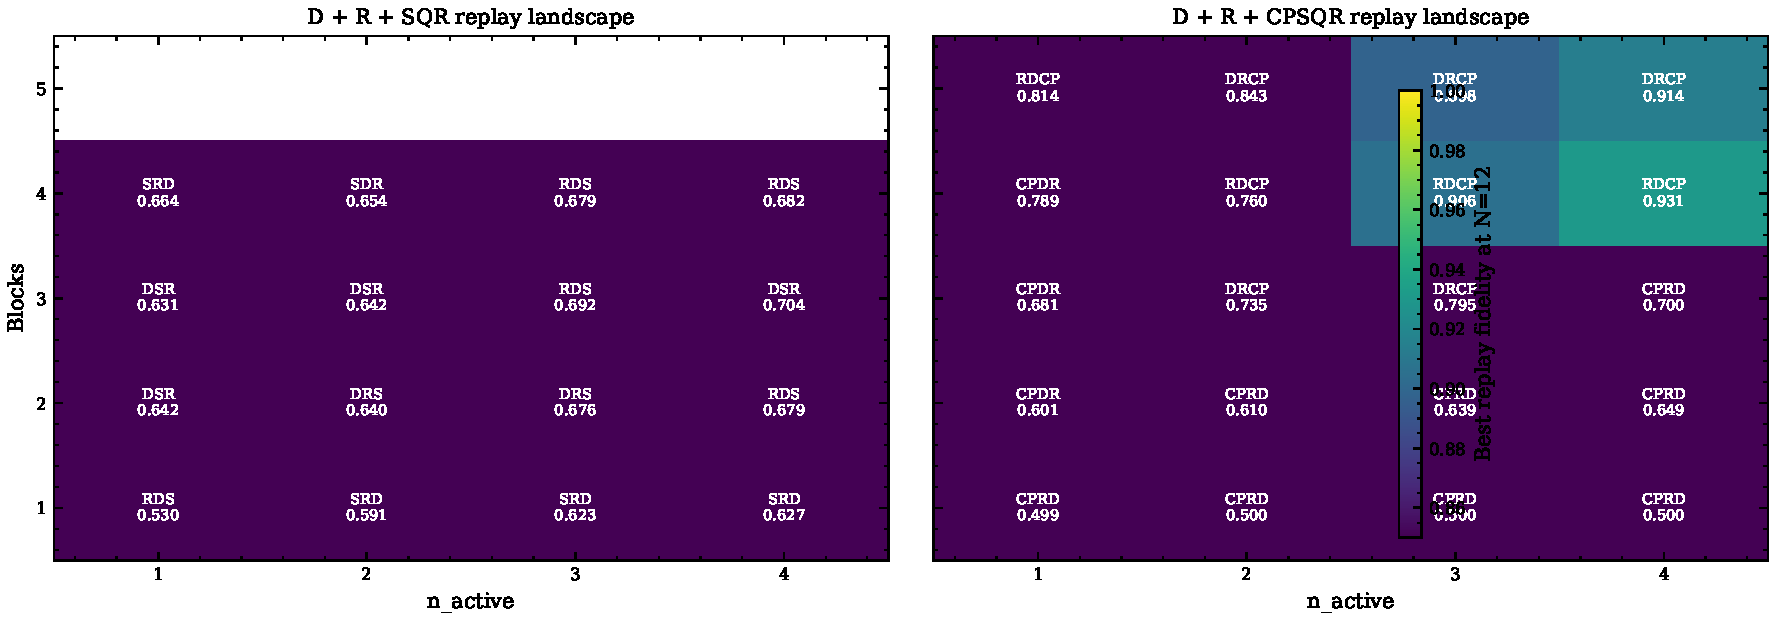
\includegraphics[width=\textwidth]{../figures/corrected_design_space_heatmaps.pdf}
\caption{Best coarse-screen replay fidelity at $N_{\mathrm{cav}}=12$ for each
$(\mathrm{blocks}, n_{\mathrm{active}})$ pair, annotated by the best ordering.
Block count is the dominant resource knob in both families.}
\label{fig:heatmaps}
\end{figure*}

\begin{figure*}[t]
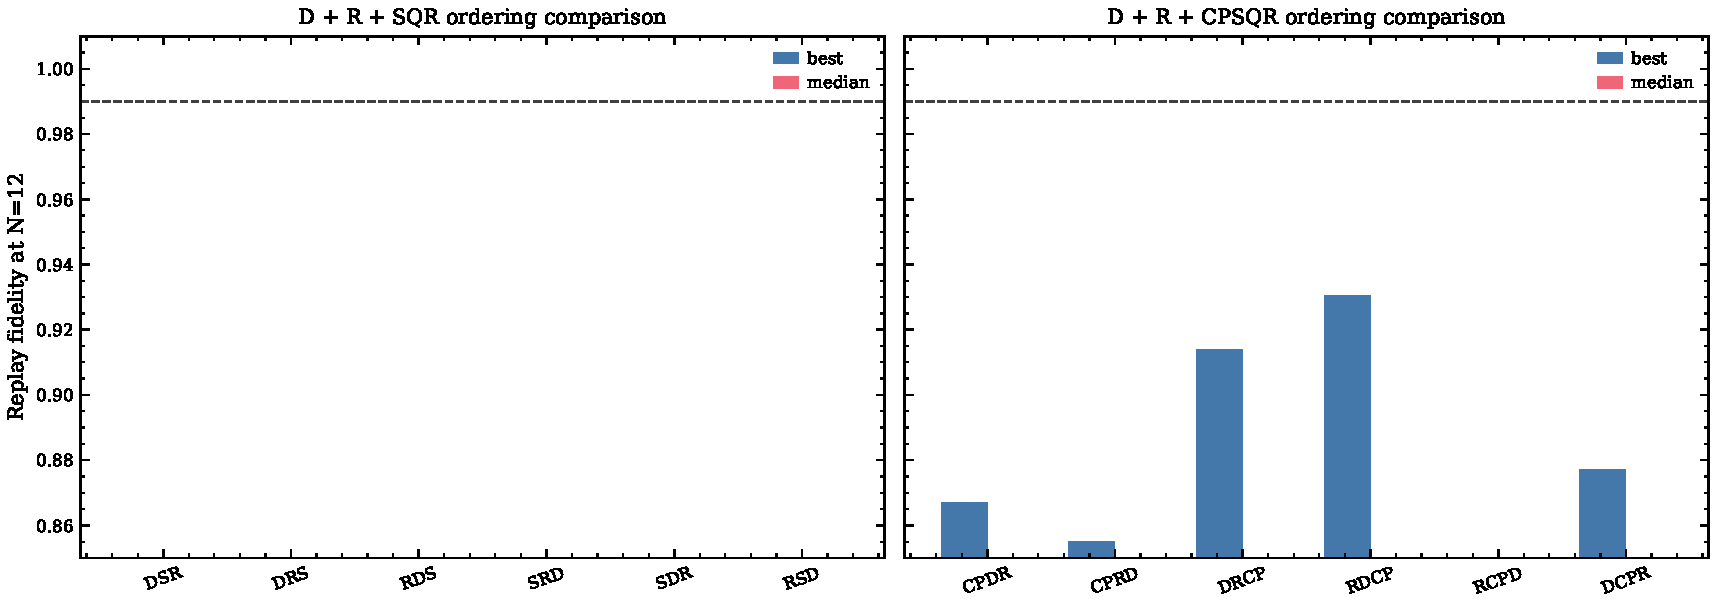
\includegraphics[width=\textwidth]{../figures/corrected_ordering_tradeoff.pdf}
\caption{Ordering tradeoffs from the coarse-screen replay data. Bars show the
best and median $N_{\mathrm{cav}}=12$ replay fidelity for each ordering within a
family. SQR has a relatively tight ordering cluster near the top, whereas
CPSQR shows a broader separation between the leading and trailing orderings.}
\label{fig:ordering}
\end{figure*}

\subsection{Physical retention at \texorpdfstring{$N_{\mathrm{cav}}=12$}{Ncav=12}}

Table~\ref{tab:physical} shows the best physically refined candidate from each
exclusive family. Unlike the earlier corrected-scope rerun, both families now
survive the active-subspace and leakage checks. The best SQR candidate is a
5-block, four-tone $RDS$ sequence acting on levels $\{0,1,2,3\}$; after the
targeted $N_{\mathrm{cav}}=12$ refinement it reaches
$F_{12}=0.9996347$ with worst logical leakage
$7.77\times 10^{-4}$ and active support bounded to levels $0$ through $3$.
The best CPSQR candidate is a 5-block, two-tone $DRCP$ sequence on levels
$\{1,2\}$; it reaches $F_{12}=0.9974917$ with worst logical leakage
$5.42\times10^{-3}$ and active support bounded to levels $0$ through $5$.

\begin{table*}[t]
\centering
\caption{Best physically refined candidate from each exclusive family.
Active levels denote the candidate-wide active subspace at the stated
truncation.}
\label{tab:physical}
\begin{tabular}{@{}lcccccccccc@{}}
\toprule
Family & Blocks & $n_{\mathrm{active}}$ & Order & Levels & $F_{10}$ & $F_{12}$ & $F_{14}$ & $L_{\mathrm{worst},12}$ & Active $N_{12}$ & Status \\
\midrule
$D+R+\mathrm{SQR}$ & 5 & 4 & RDS & $\{0,1,2,3\}$ & 0.99963 & 0.99963 & 0.99963 & $7.77\times10^{-4}$ & $0\!:\!3$ & Retained \\
$D+R+\mathrm{CPSQR}$ & 5 & 2 & DRCP & $\{1,2\}$ & 0.99749 & 0.99749 & 0.99749 & $5.42\times10^{-3}$ & $0\!:\!5$ & Retained \\
\bottomrule
\end{tabular}
\end{table*}

\begin{figure}[t]
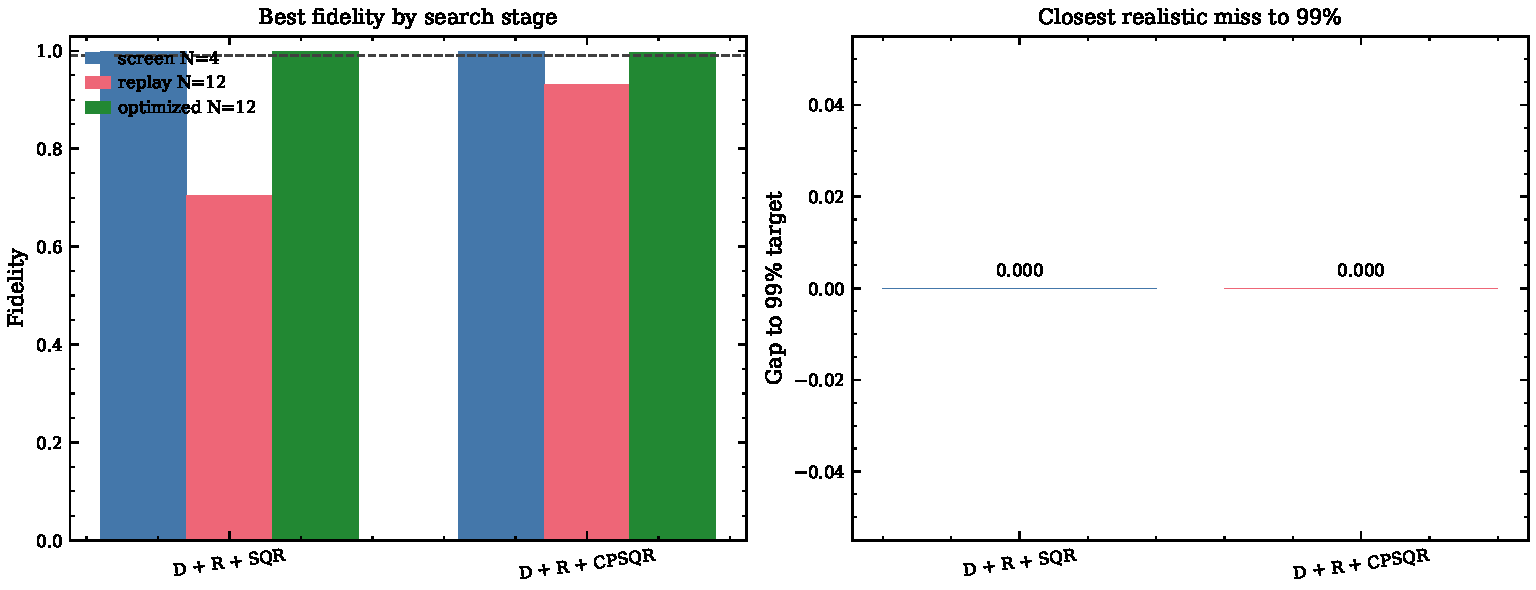
\includegraphics[width=\columnwidth]{../figures/corrected_family_tradeoff.pdf}
\caption{Structured-family comparison after the design-space refinement. Left:
best coarse-screen fidelity versus final $N_{\mathrm{cav}}=12$ refined
fidelity. Right: gap to the $99\%$ target for the best realistic candidate in
each family.}
\label{fig:tradeoff}
\end{figure}

The physical refinement changes the interpretation of the screen in two ways.
For SQR, the screen already pointed to a deep, high-tone ordering cluster; the
final refinement confirms that a 5-block $RDS$ sequence is the best closed-
system structured solution in the study. For CPSQR, by contrast, the finalist
refinement reveals that the strongest physical solution is not the coarse-
screen four-tone winner but a leaner two-tone $DRCP$ sequence on levels
$\{1,2\}$. The CPSQR family therefore trades some peak fidelity for a much
smaller tone budget and a shorter total duration.

\subsection{Active-subspace diagnostics}

Figure~\ref{fig:active} shows that both retained candidates remain well inside
the cavity basis after the final refinement. The SQR winner is the cleaner of
the two in leakage and active support, remaining concentrated on levels
$0$ through $3$. The CPSQR winner occupies a broader but still well-bounded
subspace up to level $5$.

\begin{figure}[t]
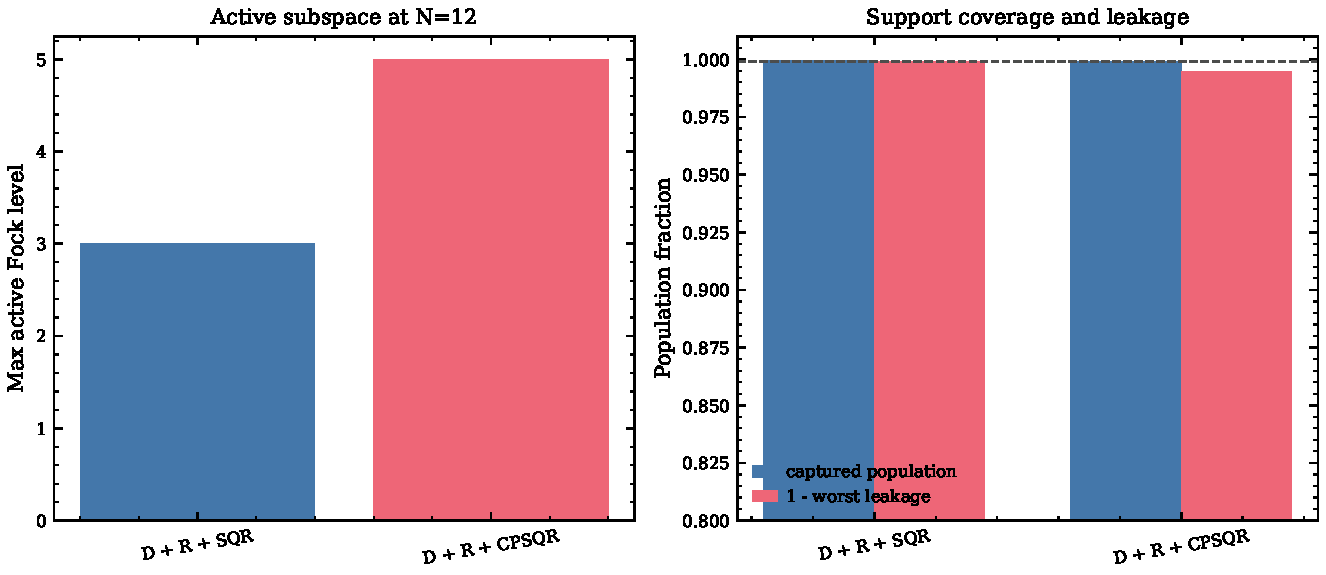
\includegraphics[width=\columnwidth]{../figures/corrected_active_subspace_summary.pdf}
\caption{Active-subspace diagnostics at $N_{\mathrm{cav}}=12$. Both retained
structured winners stay bounded inside the cavity basis. The SQR winner is more
compact in support, while the CPSQR winner occupies a somewhat broader but
still controlled subspace.}
\label{fig:active}
\end{figure}

The active-subspace diagnostic now serves a different role than in the earlier
corrected study. It is no longer a veto that eliminates SQR altogether. Rather,
it separates the two retained strategies by support footprint: the SQR winner
achieves the higher fidelity and lower leakage but needs the maximum tone
budget, whereas the CPSQR winner uses fewer tones and a shorter duration at the
cost of a broader active support and a slightly larger leakage floor.

\subsection{Ground-sector follow-up}

The reduced target changes the problem qualitatively. When the saved full-target
winners are rescored on the restricted ground-sector transfer, both collapse to
restricted fidelity near $0.50$ and ancilla excitation near unity. The old
winners are therefore not shallow approximations to the reduced task; they are
solving a different problem.

We then warm-start one representative per family and block count under the
restricted objective at \(N_{\mathrm{cav}}=12\). The resulting ranking is
summarized in Table~\ref{tab:ground_followup}. Two points are immediate. First,
both families exceed $0.99$ already at three blocks under the reduced target,
whereas the old full-target study needed at least four blocks for SQR and five
for CPSQR. Second, the best absolute reduced-objective solution is no longer the
same family-depth combination as in the full-target study: the best SQR result
is a 5-block $RDS$ sequence with
$F_{\mathrm{ground},12}=0.9999260$, while the best CPSQR result is a 4-block
$RDCP$ sequence with $F_{\mathrm{ground},12}=0.9999284$.

\begin{table*}[t]
\centering
\caption{Restricted ground-sector follow-up at \(N_{\mathrm{cav}}=12\).
\(F_{\mathrm{full},12}\) is the original full-target fidelity of the
restricted-target refined sequence, \(F_{\mathrm{ground},12}\) is the reduced
ground-sector fidelity, and \(L_{\mathrm{out},12}\) is the worst leakage out
of \(\{\ket{g,0},\ket{g,1}\}\).}
\label{tab:ground_followup}
\begin{tabular}{@{}llccccccc@{}}
\toprule
Family & Role & Blocks & $n_{\mathrm{active}}$ & Order & Levels & $F_{\mathrm{full},12}$ & $F_{\mathrm{ground},12}$ & $L_{\mathrm{out},12}$ \\
\midrule
$D+R+\mathrm{SQR}$ & Best absolute & 5 & 4 & RDS & $\{0,1,2,3\}$ & 0.3675 & 0.9999260 & $1.77\times10^{-4}$ \\
$D+R+\mathrm{SQR}$ & Minimum depth $>0.99$ & 3 & 4 & RDS & $\{0,1,2,3\}$ & 0.2948 & 0.9997453 & $5.97\times10^{-4}$ \\
$D+R+\mathrm{CPSQR}$ & Best absolute & 4 & 4 & RDCP & $\{0,1,2,3\}$ & 0.1689 & 0.9999284 & $1.76\times10^{-4}$ \\
$D+R+\mathrm{CPSQR}$ & Minimum depth $>0.99$ & 3 & 3 & DRCP & $\{0,1,2\}$ & 0.4101 & 0.9978771 & $4.20\times10^{-3}$ \\
\bottomrule
\end{tabular}
\end{table*}

Figure~\ref{fig:ground_block} shows the block-by-block comparison. The dashed
curves correspond to simply rescoring the old full-target representatives,
which stays far below threshold. The solid curves show the restricted-target
local refinements, which rise sharply and place both families above $0.99$ at
three blocks. The two-block frontier remains just sub-threshold for both
families, at $0.9875652$ for SQR and $0.9886810$ for CPSQR, making that depth
the most valuable target for the next fresh search.

\begin{figure*}[t]
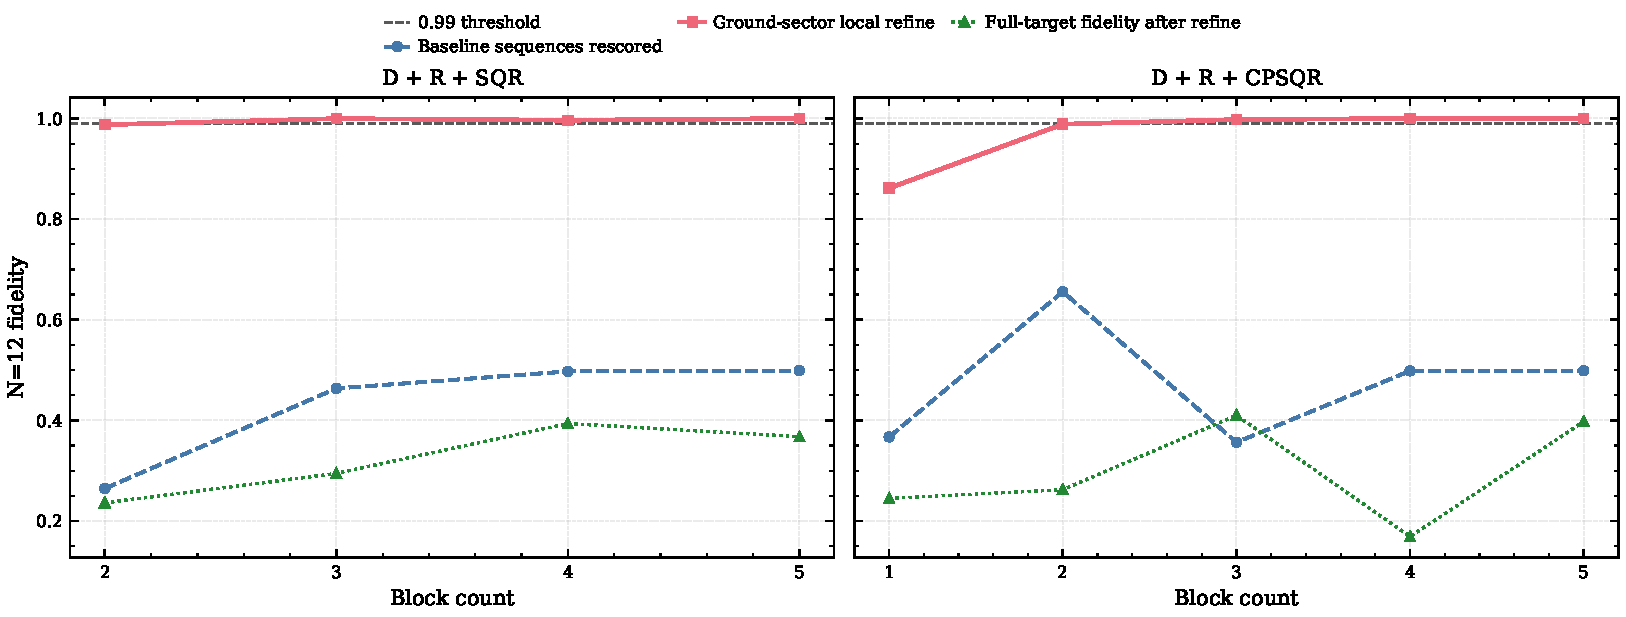
\includegraphics[width=\textwidth]{../figures/ground_sector_block_summary.pdf}
\caption{Restricted-target block comparison at \(N_{\mathrm{cav}}=12\). Dashed
curves show the old full-target block representatives rescored on the reduced
objective. Solid curves show the same representatives after local
restricted-target refinement. Both families cross the $0.99$ threshold at three
blocks, while the two-block frontier remains just below threshold.}
\label{fig:ground_block}
\end{figure*}

Figure~\ref{fig:ground_scatter} makes the more important conceptual point:
the reduced target is not a gentle relaxation of the full target. The refined
points with the best restricted fidelities sit far from the diagonal because
their full-target fidelities remain poor. The reduced objective therefore needs
its own optimization pass and should not be inferred from the full-target
ranking.

\begin{figure}[t]
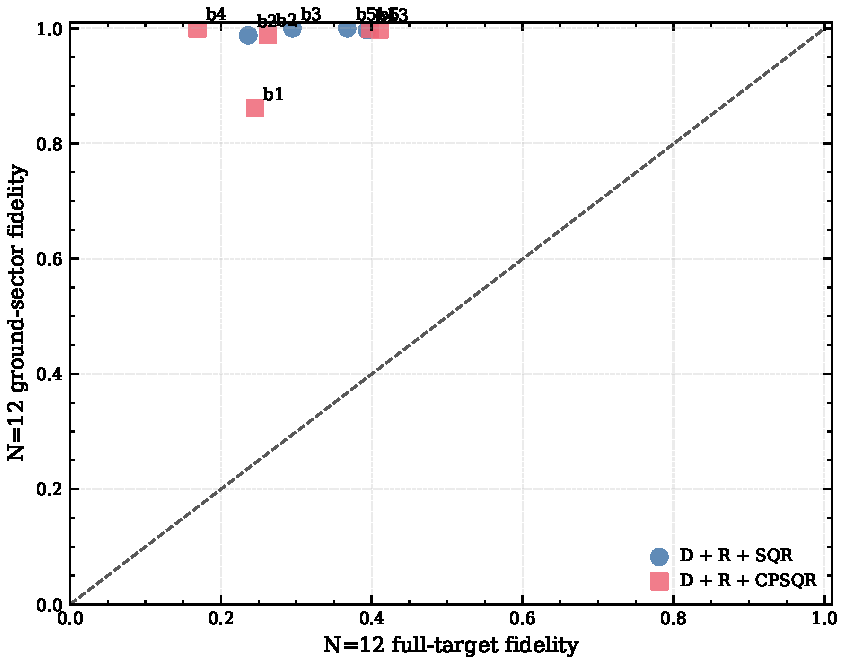
\includegraphics[width=\columnwidth]{../figures/ground_sector_objective_scatter.pdf}
\caption{Full-target versus restricted-target fidelity at
\(N_{\mathrm{cav}}=12\) for the restricted-target refined block
representatives. The best reduced-objective solutions lie far from the diagonal,
showing that the reduced task is not well approximated by the original
full-target winners.}
\label{fig:ground_scatter}
\end{figure}

\subsection{GRAPE reference}

GRAPE is kept here only as a separate reference, not as part of the structured
family ranking. The extended $N_{\mathrm{cav}}=12$ frontier now covers
\SIlist{500;600;800;1000}{ns} with identical three-seed budgets and the same
replay/open-process validation pipeline. The best replay point in that extended
scan is the \SI{800}{ns} waveform with
$F_{\mathrm{replay}} = 0.9760$, worst replay leakage
$4.34\times10^{-2}$, and open-system process fidelity
$F_{\mathrm{open}} = 0.9187$. The \SI{1000}{ns} point regresses to replay
fidelity $0.9712$ and open-process fidelity $0.9018$, so the frontier appears
to fall short of the $99\%$ replay target within the explored duration window.
Because every tested seed stops at the fixed iteration cap, this result should
be interpreted as a statement about the present durations and optimization
settings, not as evidence of a hard fidelity ceiling.
Figure~\ref{fig:grape} summarizes this extended physically validated frontier.

\begin{figure}[t]
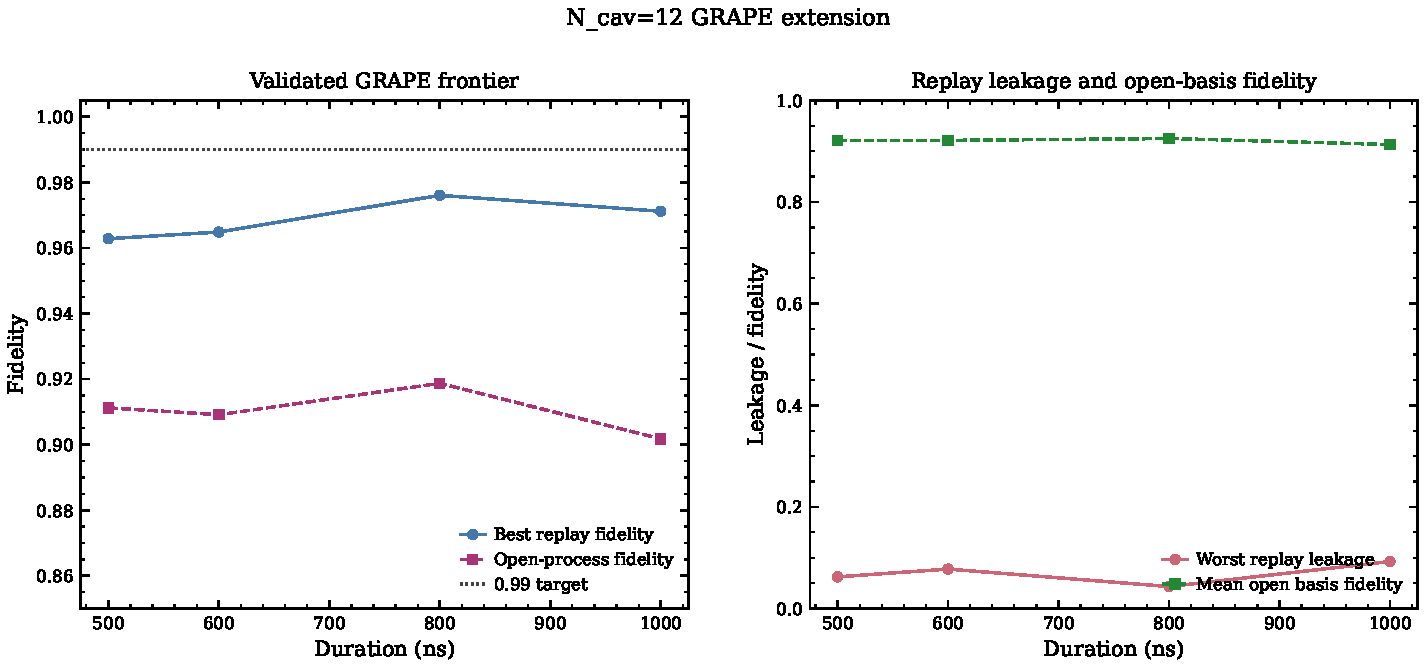
\includegraphics[width=\columnwidth]{../figures/grape_frontier_extension.pdf}
\caption{Extended physically validated full-target GRAPE frontier at
$N_{\mathrm{cav}}=12$. The replay fidelity rises from $0.9628$ at
\SI{500}{ns} to a best value $0.9760$ at \SI{800}{ns}, then falls back to
$0.9712$ at \SI{1000}{ns}. The open-system process fidelity peaks at $0.9187$
for the same \SI{800}{ns} point. No tested duration in the
\SIrange{500}{1000}{ns} window reaches the $0.99$ replay target under the
explored settings.}
\label{fig:grape}
\end{figure}

The expanded structured-family result changes the balance with respect to the
GRAPE reference. In the closed-system ideal-unitary metric, both structured
winners now exceed the GRAPE replay fidelity and cross the $99\%$ threshold.
The extended frontier sharpens that statement: the physically validated
full-target GRAPE route improves from the earlier \SI{400}{ns} point up to
\SI{800}{ns}, but under the explored durations and optimizer settings it still
does not reach replay fidelity $0.99$ in the \SIrange{500}{1000}{ns} window.
However, the structured decompositions are far slower than the validated GRAPE
pulses and still lack their own open-system process-fidelity study. The
design-space answer is therefore narrower than ``replace GRAPE'': it shows what
structured resources are sufficient to clear $99\%$ in the ideal model, not
which method is best on hardware.

\section{Validation}

\subsection{Sanity checks}

The target unitary used in the rerun was checked against the analytic
decomposition $\mathrm{SWAP}\cdot\mathrm{CZ}\cdot(H\otimes I)$ and against the
framework factory in the reproducibility notebook. Closed-system sequence
evaluation also reports machine-precision unitarity errors for the structured
candidates.

\subsection{Convergence analysis}

The corrected study still does not accept any final conclusion from
$N_{\mathrm{cav}}\leq 8$. Instead, the best refined candidate from each
exclusive family is re-evaluated at $N_{\mathrm{cav}}=10,12,14$.

The SQR winner is numerically stable to the shown precision:
$F_{10}=0.9996347$, $F_{12}=0.9996347$, $F_{14}=0.9996347$, with worst logical
leakage staying near $7.8\times10^{-4}$ and the active support fixed at levels
$0$ through $3$.

The CPSQR winner is likewise stable:
$F_{10}=0.9974917$, $F_{12}=0.9974917$, $F_{14}=0.9974917$, with worst logical
leakage near $5.4\times10^{-3}$ and active support fixed at levels $0$ through
$5$.

The main convergence lesson is therefore no longer ``discard SQR.'' Instead it
is that the staged search must be followed by explicit high-truncation
re-optimization. The earlier corrected-scope conclusion was too pessimistic
because it stopped short of this final refinement step.

The same conclusion applies even more strongly to the restricted-target branch.
The refined 3-block and best-absolute reduced-objective candidates remain
stable across \(N_{\mathrm{cav}}=10,12,14\). For SQR, the 3-block winner stays
at $F_{\mathrm{ground}}\approx0.999745$ with outside-target leakage below
$6\times10^{-4}$. For CPSQR, the 4-block best-absolute winner stays at
$F_{\mathrm{ground}}\approx0.999928$ with outside-target leakage below
$2\times10^{-4}$. The two-block representatives remain sub-threshold but are
also numerically stable, so the next uncertainty is search completeness at low
depth rather than truncation drift.

\subsection{Comparison to prior validated reference}

This study is not a literature-reproduction task. The closest external point of
comparison is the previously validated GRAPE follow-up within the same research
program. The corrected structured-family conclusion is consistent with that
reference in two ways. First, the structured sequences are much longer than the
GRAPE pulse, so any hardware comparison must include decoherence. Second, the
structured winners now beat the GRAPE replay fidelity in the ideal closed-
system metric, which means the remaining question is no longer whether the
structured approach can reach $99\%$, but whether it can do so under realistic
noise within an acceptable duration.

There is also a third route, but only at the primitive level so far. The
third route is now characterized directly inside this unified study by
optimizing representative retained primitives with qubit-only GRAPE and
replaying them on cavity probe states. We selected the first retained SQR block
($S0$) and the longest retained CPSQR block ($CP2$), optimized each on the
diagnostic subspace most relevant to its addressed levels, and then compared
the replayed pulse against the corresponding ideal primitive action on both the
full joint state and the reduced cavity state. Figures~\ref{fig:primitive_summary}
and \ref{fig:primitive_wigner} collect the resulting primitive-level
diagnostics. The representative SQR primitive is clearly the stronger
precursor, but it is still not hybrid-ready: it reaches only
$F_{\mathrm{sub}}=0.6959$, with mean full-state probe fidelity $0.5793$ and
mean reduced-cavity fidelity $0.8429$. The representative CPSQR primitive is
weaker still, reaching $F_{\mathrm{sub}}=0.4754$, with mean full-state probe
fidelity $0.2892$ and mean reduced-cavity fidelity $0.5948$. The cavity-state
comparison is therefore materially more forgiving than the full joint-state
diagnostic, yet neither primitive is accurate enough to be inserted into the
cluster-state ansatz as a completed end-to-end third route.

\section{Discussion}

Four points emerge from the completed design-space study.

First, the earlier corrected-scope conclusion was not a fundamental limit of
the exclusive structured families. It was a limit of an incomplete search.
Once the design space is expanded over block count, tone budget, and ordering,
and the strongest candidates are re-optimized at $N_{\mathrm{cav}}=12$, both
families cross the $99\%$ target with bounded active support.

Second, block count is the dominant resource knob in both families. The effect
is modest but still leading in SQR, and decisive in CPSQR. This means that any
future structured search that fixes depth too early is likely to miss the best
family behavior.

Third, the two families reach the target in qualitatively different ways. SQR
achieves the highest fidelity, lowest leakage, and smallest active support, but
it requires the maximum four-tone budget and the longest sequence in the study.
CPSQR reaches a slightly lower fidelity yet uses only two active tones in its
best final form. If implementation complexity is measured by tone budget, the
CPSQR winner is the more economical design; if it is measured by ideal closed-
system fidelity, the SQR winner is superior.

Fourth, ordering matters, but its role depends on whether one emphasizes robust
screen behavior or best-case refined performance. The SQR screen medians favor
DSR, yet the top refined solution uses RDS. The CPSQR screen medians favor
CPDR, while the best refined solution is DRCP. In other words, the best robust
ordering and the best ultimately refinable ordering need not coincide.

Fifth, the reduced ground-sector objective is not simply a softened version of
the full logical target. The old full-target winners fail badly on the reduced
task because they rely on ancilla excitation that is irrelevant or even harmful
for the cavity-only transfer. Once the objective is changed, both the minimum
depth and the winning family-depth combination change as well: both families now
reach the threshold at three blocks, and the best absolute reduced-objective
point is a 4-block CPSQR candidate rather than the 5-block full-target SQR
winner.

\section{Conclusion}

Under the corrected family scope and the completed two-branch analysis, the
answer is now more specific than in the earlier rerun.

\begin{enumerate}
  \item The structured-family comparison must be limited to
  $D+R+\mathrm{SQR}$ and $D+R+\mathrm{CPSQR}$ only.
  \item Final conclusions must still be drawn from $N_{\mathrm{cav}}>8$, with
  $N_{\mathrm{cav}}=12$ as the default evidence level.
  \item For the full-target branch, the best pure SQR solution is a 5-block,
  four-tone $RDS$ sequence on
  levels $\{0,1,2,3\}$ with
  $F_{12}=0.9996347$ and worst leakage $7.77\times10^{-4}$.
  \item For the full-target branch, the best pure CPSQR solution is a 5-block,
  two-tone $DRCP$ sequence on
  levels $\{1,2\}$ with
  $F_{12}=0.9974917$ and worst leakage $5.42\times10^{-3}$.
  \item Both exclusive structured families therefore reach the $99\%$ target
  under the closed-system ideal-unitary metric.
  \item For the reduced ground-sector branch, the old full-target winners are
  not competitive: their restricted fidelities fall to about $0.50$ because
  they excite the ancilla almost completely.
  \item After restricted-target local refinement, both families reach the
  $0.99$ threshold already at three blocks. The best absolute reduced-target
  solutions are a 5-block SQR $RDS$ sequence with
  $F_{\mathrm{ground},12}=0.9999260$ and a 4-block CPSQR $RDCP$ sequence with
  $F_{\mathrm{ground},12}=0.9999284$.
  \item The two-block restricted-target frontier remains just below threshold
  in both families, so the next high-value search should start there.
  \item Blocks remain the dominant structural driver in both branches, but the
  reduced objective changes which family-depth combination wins.
  \item Direct GRAPE remains the faster and more physically validated route,
  but the extended $N_{\mathrm{cav}}=12$ frontier does \emph{not} reach replay
  fidelity $0.99$ up to \SI{1000}{ns}; its best tested point is
  \SI{800}{ns} with replay fidelity $0.9760$ and open-system process fidelity
  $0.9187$.
  \item Primitive-level GRAPE diagnostics do not yet furnish a finished hybrid
  third route. The representative SQR block reaches only
  $F_{\mathrm{sub}}=0.6959$ with mean reduced-cavity fidelity $0.8429$, while
  the representative CPSQR block reaches $F_{\mathrm{sub}}=0.4754$ with mean
  reduced-cavity fidelity $0.5948$.
\end{enumerate}

The concise recommendation is therefore layered. If the objective is the full
joint logical map, keep the 5-block SQR and 5-block CPSQR winners from the
baseline branch. If the objective is the reduced cavity-only transfer on the
ground ancilla sector, do not reuse those solutions; use the dedicated
restricted-target winners instead, with the 3-block representatives as the
current minimum-depth branch and the 4-block CPSQR point as the best absolute
restricted-target solution. If the objective is the fastest route with existing
open-system validation, full-target GRAPE remains preferred, with the current
best validated point at \SI{800}{ns}. If the objective is to identify which
selective primitive is most promising for a future hybrid ansatz, the present
representative primitive diagnostics still favor SQR over CPSQR, but neither
primitive is yet accurate enough to act as a drop-in replacement for the ideal
selective block.

For the next optimization stage, the search priority should be reordered again.
The highest-value unresolved question is now the fresh 2-block restricted-target
frontier. Only after that low-depth threshold is resolved should the search
systematically reduce $n_{\mathrm{active}}$ and then refine duration, leakage,
and Wigner agreement. Tone-count reduction remains best treated as a follow-up
compression problem rather than the primary axis.

\section{Limitations and Future Work}

\subsection{Known Limitations}

The structured-family search is still staged: a broad screen is run at
$N_{\mathrm{cav}}=4$, exact level-subset refinement is applied only to the
strongest structures, and direct $N_{\mathrm{cav}}=12$ optimization is reserved
for the final shortlist. A fully exhaustive search performed directly at
$N_{\mathrm{cav}}=12$ is still out of reach.

The structured winners are validated only in the closed-system ideal-unitary
metric. They do not yet have the open-system process-fidelity validation that
already exists for the GRAPE reference.

The current restricted-target winners show that both families can exceed $99\%$
at three blocks in the closed-system metric, but they do not yet establish
whether a fresh two-block restricted-target search can also cross the same
threshold. That low-depth frontier is still open.

The extended full-target GRAPE replay frontier does not yet reach the $99\%$
target in the explored \SIrange{500}{1000}{ns} window. Every tested seed
terminates at the fixed iteration limit, so the present frontier constrains the
current implementation settings rather than demonstrating a model-level ceiling.

The strongest SQR winner is also the slowest solution in the final retained set
(\SI{6180}{ns}), so its hardware relevance depends sensitively on decoherence
times and calibration overhead.

\subsection{Suggested Improvements}

\begin{itemize}
  \item \textbf{[P1 | MEDIUM]} Recast the next structured search around the
  minimum block count that reaches the chosen validation metric at $99\%$.
  For the reduced ground-sector branch, this now means a fresh 2- and 3-block
  search rather than more warm-started refinement from the full-target winners.
  \item \textbf{[P1 | HIGH]} Once a depth-minimal structured candidate is
  identified, perform open-system validation for the retained winners,
  especially the 3-block restricted-target winners and the \SI{6180}{ns} SQR
  full-target sequence, and compare their process fidelities directly against
  the validated GRAPE pulse.
  \item \textbf{[P2 | MEDIUM]} Re-run the strongest SQR and CPSQR structures
  directly at $N_{\mathrm{cav}}=12$ from scratch within the selected depth,
  not only through the staged warm-start path, to check for shorter or even
  higher-fidelity solutions in both the full-target and reduced-target branches.
  \item \textbf{[P2 | MEDIUM]} Confirm the local ordering rankings with a
  second refinement budget or seed set, especially RDS versus DSR for SQR and
  DRCP versus RDCP/CPDR for CPSQR. The fixed-budget SQR rerun now clearly
  disfavors DRS, but the ordering sensitivity should still be stress-tested.
  \item \textbf{[P2 | MEDIUM]} After the minimum depth is fixed, search for
  smaller active-tone sets and then refine duration, leakage, and Wigner
  agreement. Tone-count reduction should be treated as a follow-up compression
  step rather than the primary axis.
  \item \textbf{[P2 | MEDIUM]} Add a local waveform-to-state pipeline for the
  validated GRAPE reference so the appendix can compare retained structured and
  pulse-level Wigner functions on the same footing.
  \item \textbf{[P2 | MEDIUM]} Test replay-aware or noise-aware GRAPE
  objectives, preferably with the JAX engine enabled for the current frontier
  runner. The present GRAPE frontier improves only to replay fidelity $0.9760$
  at \SI{800}{ns} and remains iteration-limited across all tested seeds.
  \item \textbf{[P2 | LOW]} Promote the active-subspace diagnostic into shared
  study utilities or upstream it into \texttt{cqed\_sim} support code.
\end{itemize}

\subsection{Open Questions}

Why do the full-target winners fail so completely on the reduced ground-sector
task, and can the two-block restricted-target frontier cross $0.99$ once it is
searched directly rather than warm-started from the old solutions? Why does the
SQR family switch from the best screen-median ordering (DSR) to the best fully
refined ordering (RDS), and why does CPSQR ultimately prefer a two-tone DRCP or
three-tone DRCP/RDCP structure depending on the objective? Answering these
questions may reveal whether the best final structured sequences are exploiting
qualitatively different control regimes in the full-target and reduced-target
branches. A second open question still comes from the Wigner analysis: if
enlarged spectator-constrained re-fits make both families worse, what physical
mechanism is actually responsible for the residual phase-space mismatch?

\bibliographystyle{apsrev4-2}
\bibliography{references}

\appendix

\section{Detailed Results and Data}

\subsection{Target observables}

Figure~\ref{fig:obs} shows the exact transmon and cavity observables for the
target output states. These are unchanged by the corrected family scope, but
they remain the reference signatures for any candidate implementation.

\begin{figure}[H]
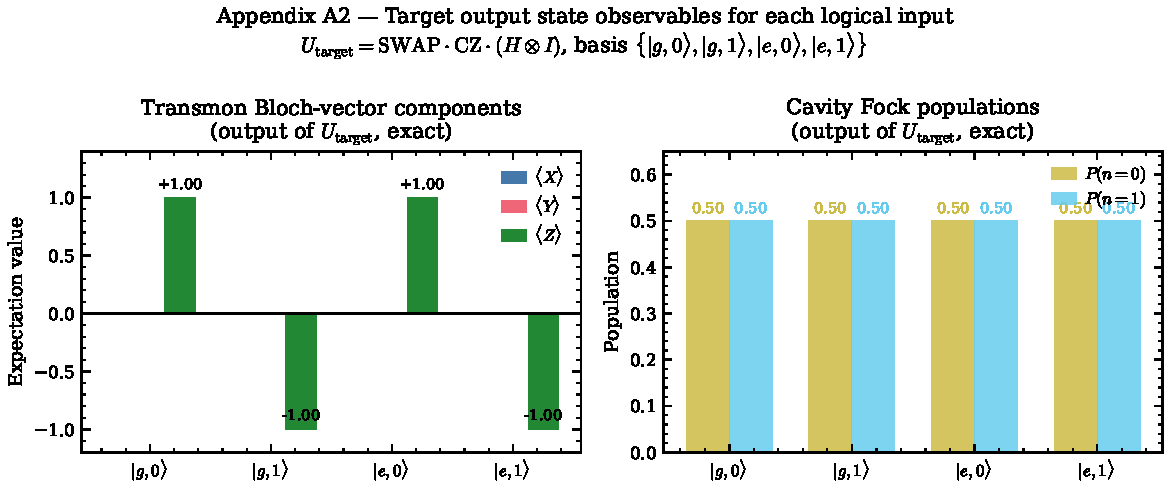
\includegraphics[width=\columnwidth]{../figures/appendix_state_observables.pdf}
\caption{Exact target output observables for the four logical inputs.}
\label{fig:obs}
\end{figure}

\subsection{Corrected Wigner appendix}

Figure~\ref{fig:wigner} now uses a single local figure directory and only shows
the target state together with the best retained SQR and CPSQR candidates. No
mixed-family panels appear.

\begin{figure*}[t]
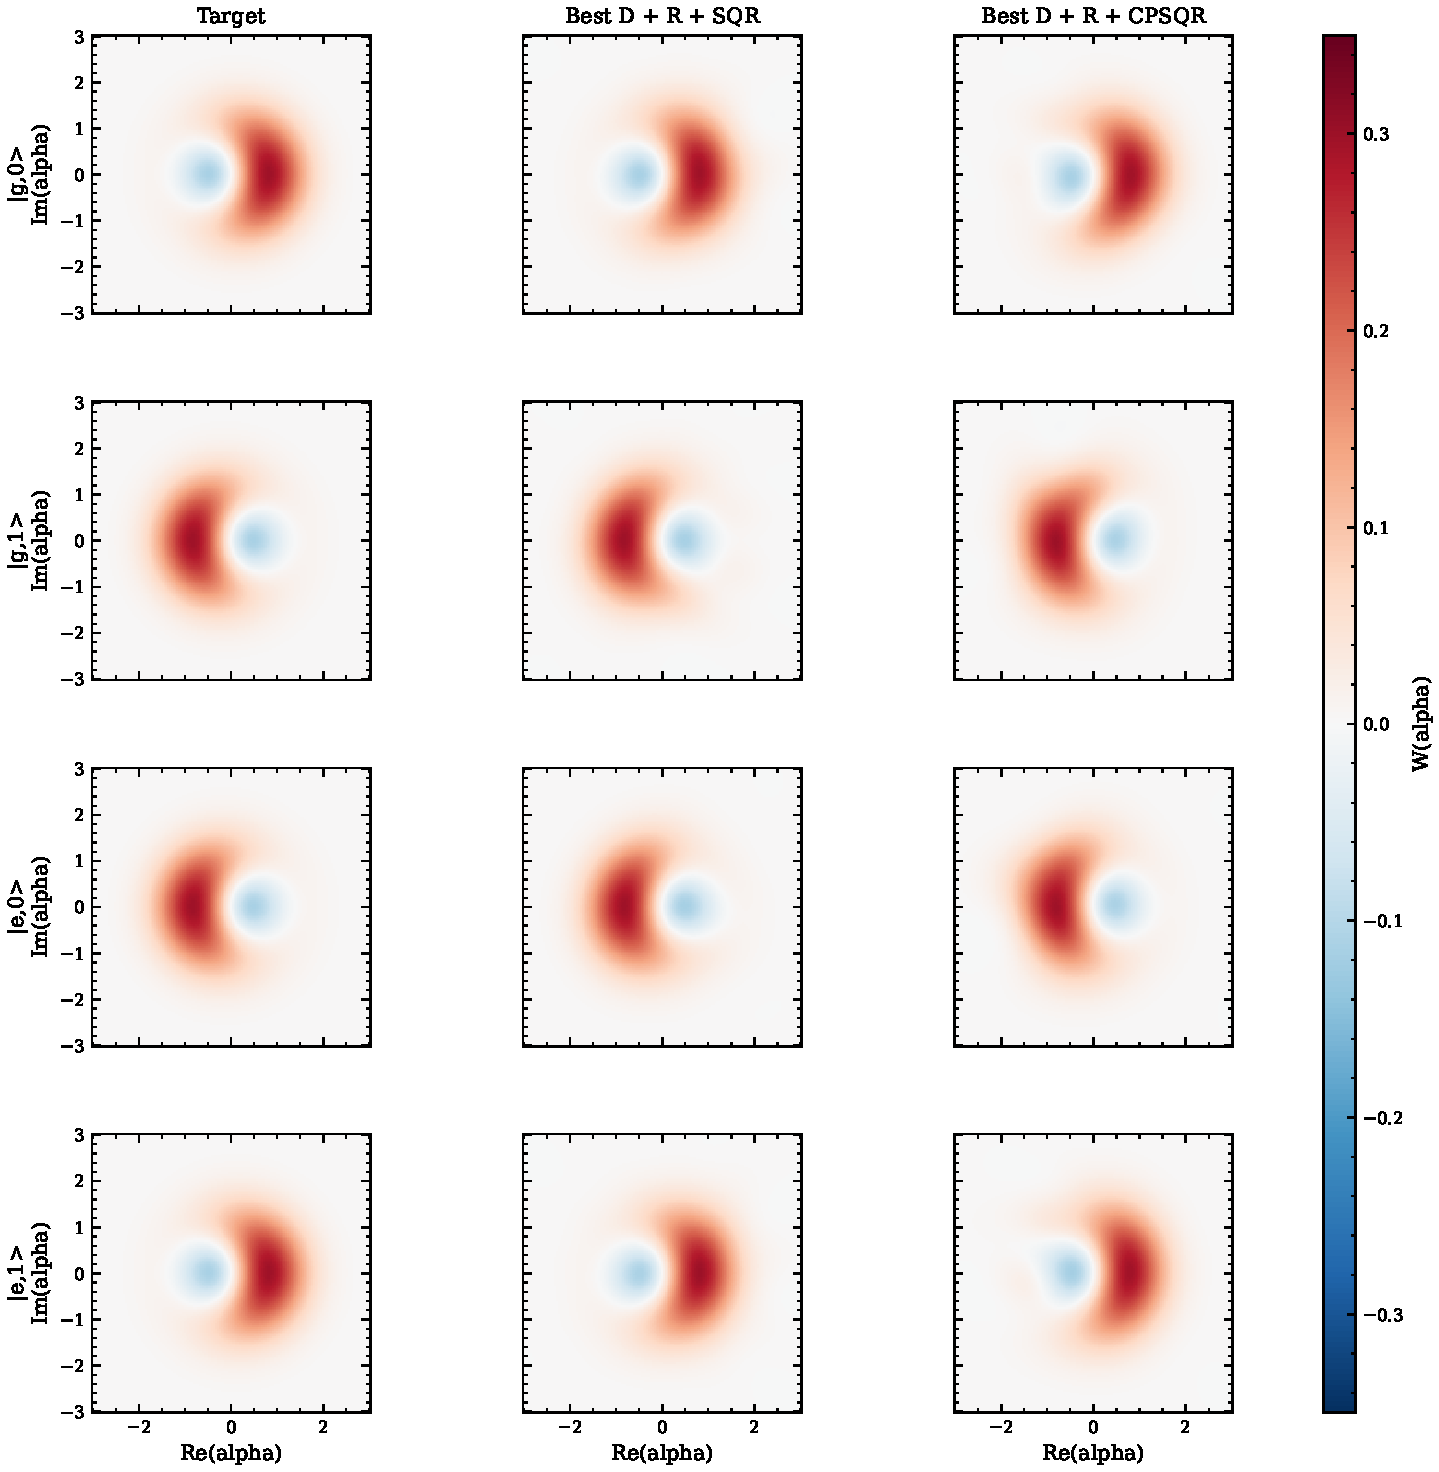
\includegraphics[width=\textwidth]{../figures/appendix_wigner.pdf}
\caption{Appendix Wigner panels from the comprehensive design-space study. The
figure shows the target state together with the best retained
$D+R+\mathrm{SQR}$ and $D+R+\mathrm{CPSQR}$ candidates.}
\label{fig:wigner}
\end{figure*}

\subsection{Primitive-level GRAPE diagnostics}

To make the primitive-level ``third route'' concrete within the same study, we
optimized one representative retained block from each family with qubit-only
GRAPE and compared the replayed action against the corresponding ideal
primitive on probe states. The retained SQR representative is the first
selective block $S0$ from the final 5-block $RDS$ winner; the retained CPSQR
representative is the longest conditional-phase block $CP2$ from the final
5-block $DRCP$ winner. The optimization target is restricted to the diagnostic
level subspace relevant to the probe states, while the replay and probe-state
comparison are evaluated at $N_{\mathrm{cav}}=12$.

Figure~\ref{fig:primitive_summary} shows the optimized waveforms and the direct
probe-state fidelity comparison. The SQR primitive preserves the reduced cavity
state noticeably better than the full joint state, but even its best replay is
still far from ideal on the full probe set. The CPSQR primitive is weaker and,
most importantly, fails on its addressed $\{1,2\}$ probe rather than only on a
spectator-dominated input. Figure~\ref{fig:primitive_wigner} shows the reduced
cavity Wigner comparison on the worst reduced-cavity probe for each primitive.
These state-level diagnostics make clear that the present primitive GRAPE runs
are useful as diagnostics, not yet as drop-in building blocks for the
structured cluster-state ansatz.

\begin{figure*}[t]
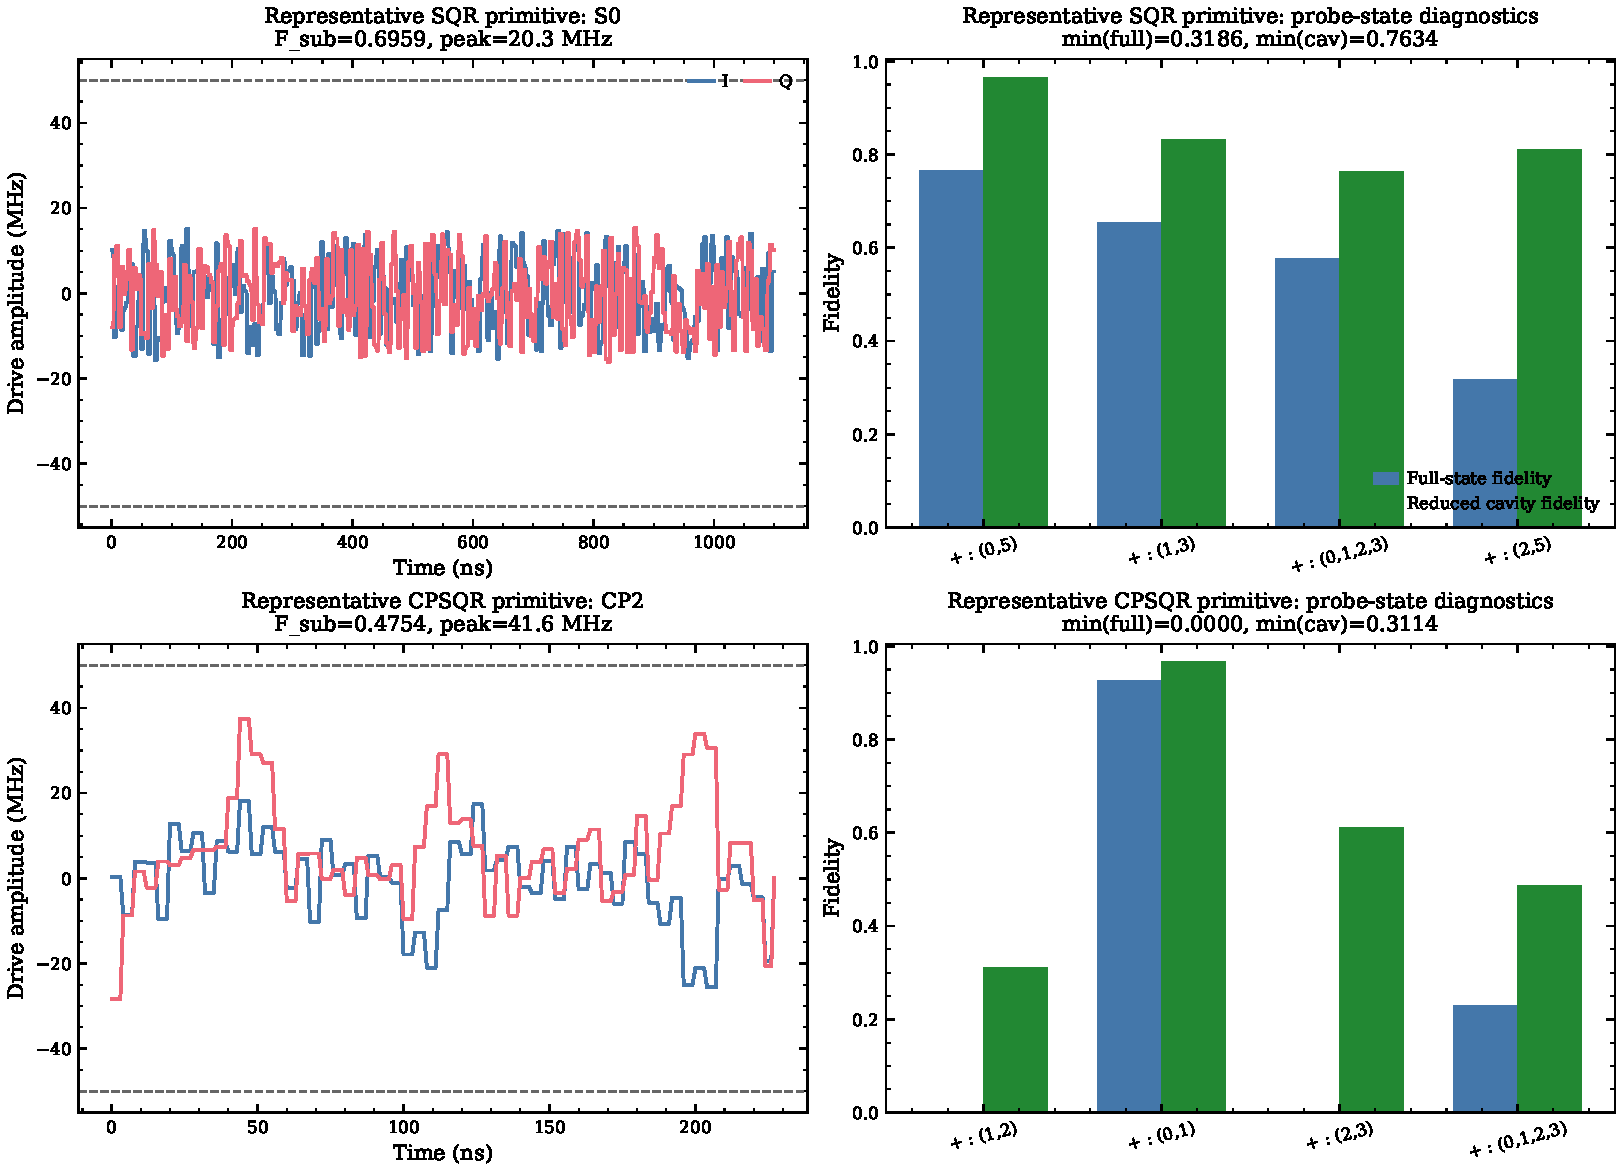
\includegraphics[width=\textwidth]{../figures/primitive_grape_summary.pdf}
\caption{Representative primitive-level GRAPE diagnostics for the retained
exclusive-family winners. Left column: optimized qubit-drive envelopes for the
selected $S0$ and $CP2$ primitives, shown in MHz with dashed lines marking the
$\pm\SI{50}{MHz}$ amplitude bound. Right column: probe-state fidelities versus
the corresponding ideal primitive action. The representative SQR primitive
reaches $F_{\mathrm{sub}}=0.6959$ with mean full-state and reduced-cavity probe
fidelities $0.5793$ and $0.8429$, respectively. The representative CPSQR
primitive reaches $F_{\mathrm{sub}}=0.4754$ with mean full-state and reduced-
cavity probe fidelities $0.2892$ and $0.5948$, respectively.}
\label{fig:primitive_summary}
\end{figure*}

\begin{figure*}[t]
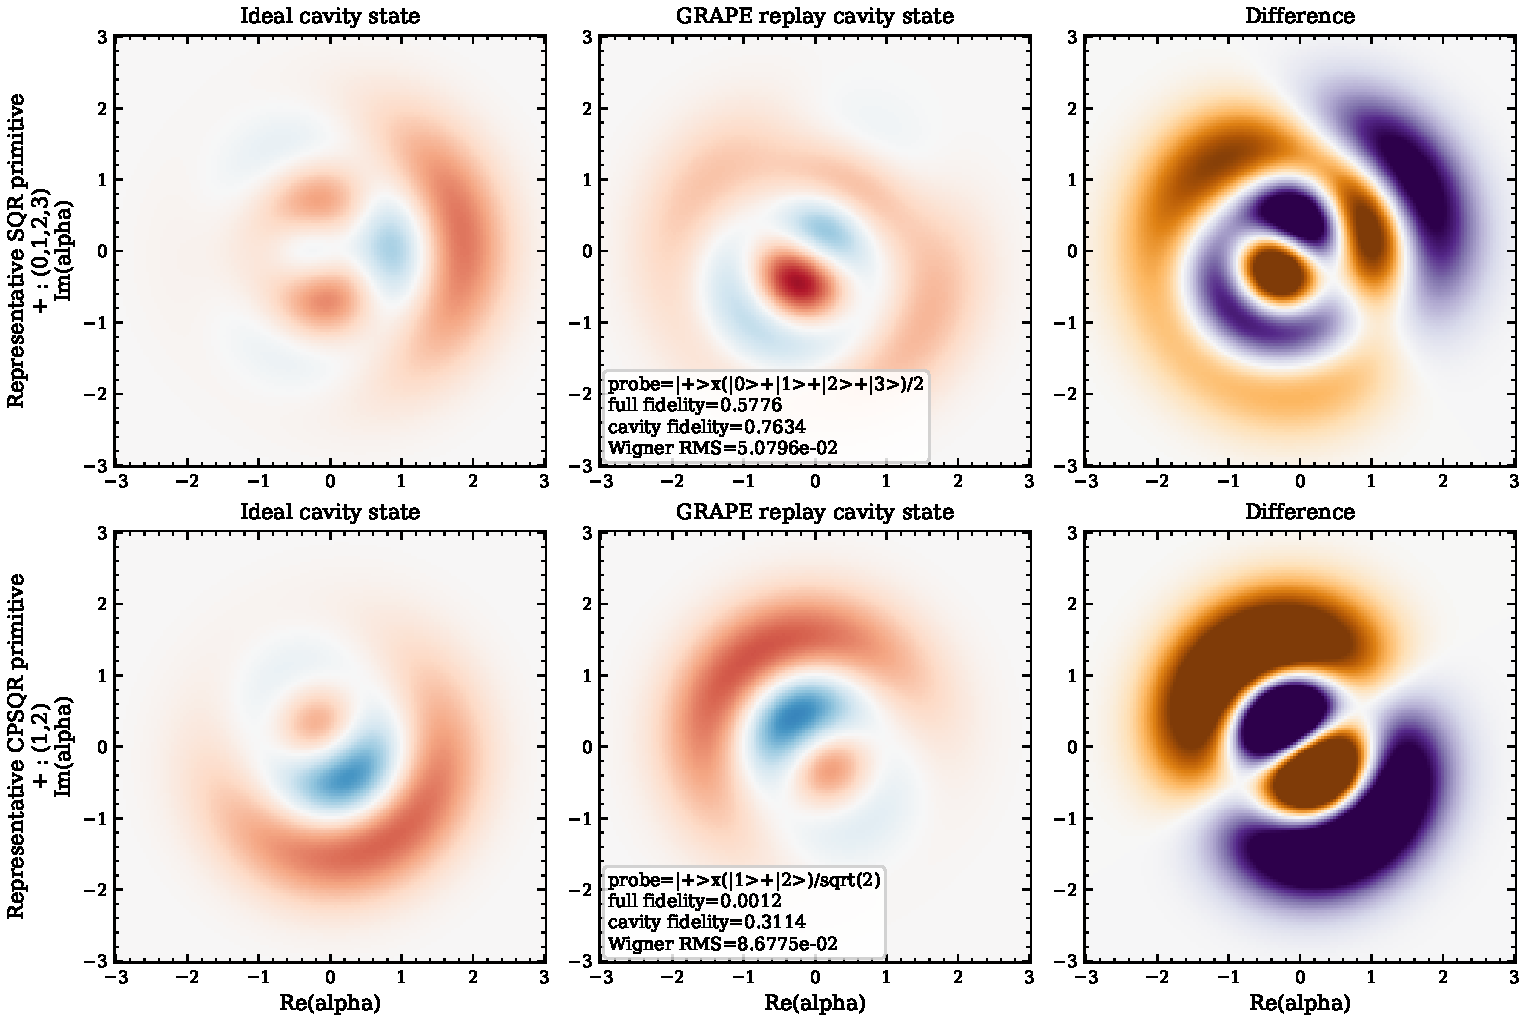
\includegraphics[width=\textwidth]{../figures/primitive_grape_wigner.pdf}
\caption{Reduced-cavity Wigner comparison on the worst reduced-cavity probe for
each representative primitive. Top: the retained SQR primitive $S0$ evaluated
on $\ket{+}\otimes(\ket{0}+\ket{1}+\ket{2}+\ket{3})/2$, where the replayed
primitive reaches full-state fidelity $0.5776$ and reduced-cavity fidelity
$0.7634$. Bottom: the retained CPSQR primitive $CP2$ evaluated on
$\ket{+}\otimes(\ket{1}+\ket{2})/\sqrt{2}$, where the replayed primitive falls
to full-state fidelity $0.0012$ and reduced-cavity fidelity $0.3114$. The
phase-space mismatch is therefore moderate for SQR and severe for CPSQR.}
\label{fig:primitive_wigner}
\end{figure*}

\subsection{Spectator-constrained Wigner test}

The residual Wigner mismatch was probed by re-optimizing each retained family
against an augmented target that also constrains spectator sectors. That test
does \emph{not} support the hypothesis that the mismatch is caused primarily by
unconstrained spectator action. For the retained
$D+R+\mathrm{SQR}$ winner, the deeper logical-only re-fit stays excellent
($F_{12}=0.999641$, mean Wigner RMS $2.04\times10^{-3}$), whereas the
augmented re-fit degrades to $F_{12}=0.887459$ with mean Wigner RMS
$1.88\times10^{-2}$. For the retained $D+R+\mathrm{CPSQR}$ winner, the
deepest complete local run uses a mixed backend path; even there the logical
re-fit remains strong ($F_{12}=0.997589$, mean Wigner RMS
$4.70\times10^{-3}$) while the augmented re-fit falls to
$F_{12}=0.868868$ with mean Wigner RMS $2.82\times10^{-2}$.

\begin{figure*}[t]
\centering
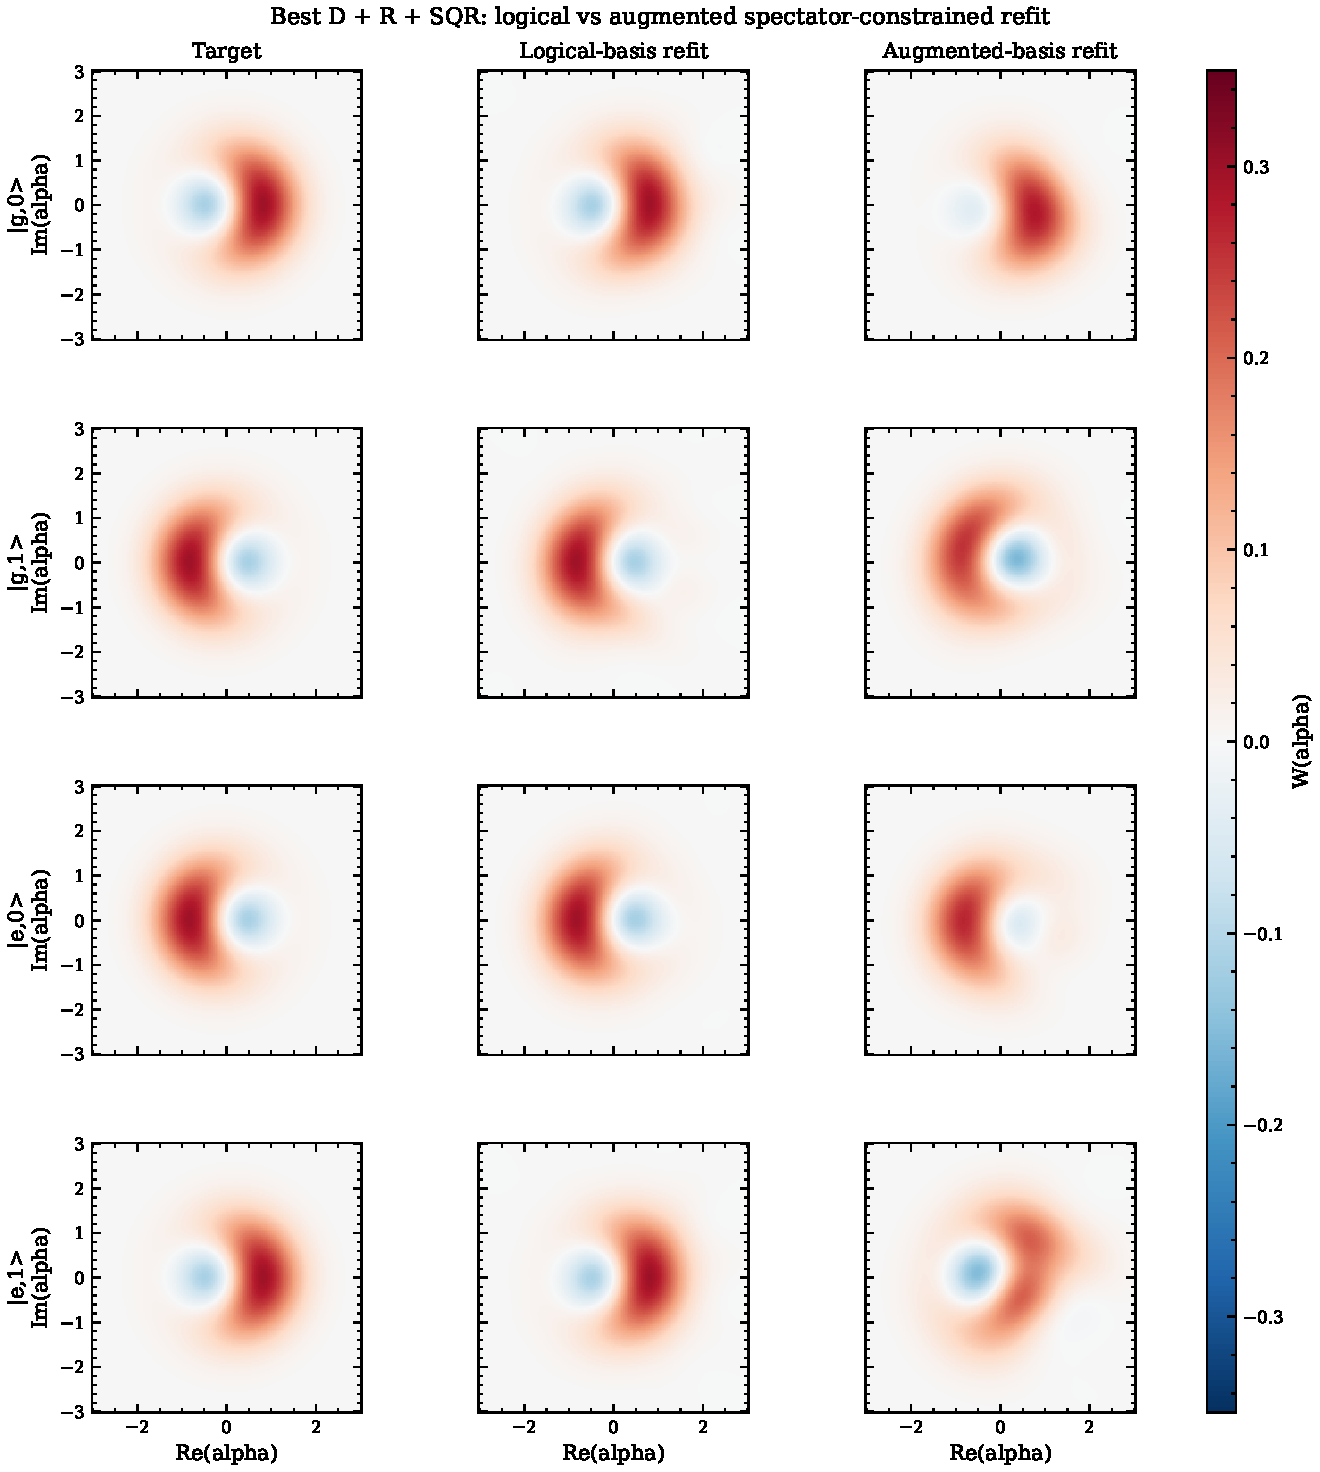
\includegraphics[width=0.49\textwidth]{../figures/drsqr_wigner_basis_extension.pdf}
\hfill
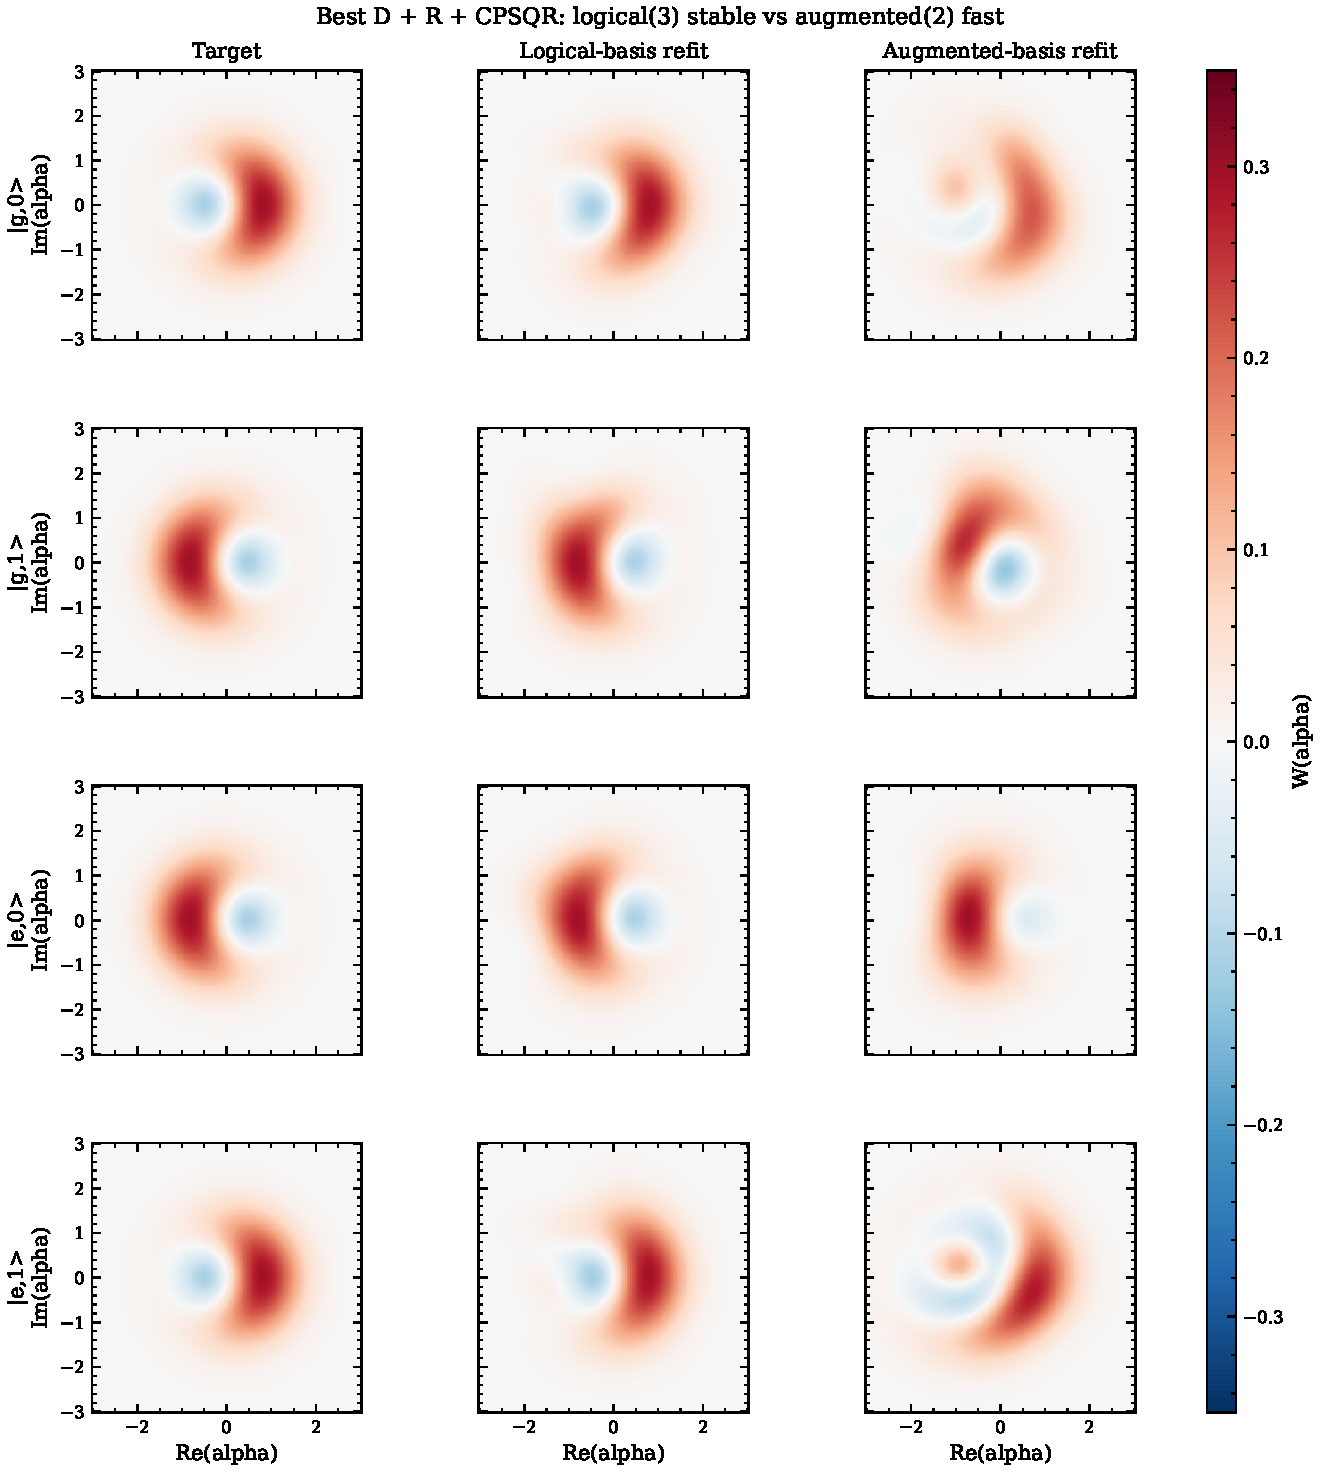
\includegraphics[width=0.49\textwidth]{../figures/drcpsqr_wigner_basis_extension_3x2mix.pdf}
\caption{Deeper spectator-constrained Wigner tests for the retained exclusive
families. Left: the retained $D+R+\mathrm{SQR}$ winner. Right: the deepest
complete local $D+R+\mathrm{CPSQR}$ test, which uses a mixed backend path for
numerical stability. In both families the spectator-constrained augmented
target worsens both fidelity and phase-space agreement rather than improving
them.}
\label{fig:wigner_basis_extension}
\end{figure*}

\section{Reproducibility}

\subsection{Optimized Parameters}

The full gate-by-gate parameters for the retained structured winners are listed
here so the paper itself, not only the machine-readable artifacts, records the
optimized schedules.

\subsubsection{Retained $D+R+\mathrm{SQR}$ winner}

This winner uses five selective blocks, four active tones, $RDS$ ordering, and
addresses levels $\{0,1,2,3\}$.

{\small
\begin{flushleft}
\textbf{R0}: QubitRotation, $40.0$ ns; $\theta=0.730$, $\phi=0.388$; addressed levels: not applicable.\\
\textbf{D0}: Displacement, $80.0$ ns; $\mathrm{Re}(\alpha)=-0.119$, $\mathrm{Im}(\alpha)=0.302$; addressed levels: not applicable.\\
\textbf{S0}: MaskedSQR, $1100.0$ ns; $\theta=[-1.879,-1.875,-1.834,1.486]$, $\phi=[-1.765,1.916,1.689,-1.483]$; addressed levels $0,1,2,3$.\\
\textbf{R1}: QubitRotation, $40.0$ ns; $\theta=1.486$, $\phi=1.596$; addressed levels: not applicable.\\
\textbf{D1}: Displacement, $80.0$ ns; $\mathrm{Re}(\alpha)=-0.015$, $\mathrm{Im}(\alpha)=-0.469$; addressed levels: not applicable.\\
\textbf{S1}: MaskedSQR, $1100.0$ ns; $\theta=[2.362,-2.107,-2.221,-2.012]$, $\phi=[-0.427,0.210,-0.255,-0.506]$; addressed levels $0,1,2,3$.\\
\textbf{R2}: QubitRotation, $40.0$ ns; $\theta=1.829$, $\phi=0.237$; addressed levels: not applicable.\\
\textbf{D2}: Displacement, $80.0$ ns; $\mathrm{Re}(\alpha)=0.285$, $\mathrm{Im}(\alpha)=0.295$; addressed levels: not applicable.\\
\textbf{S2}: MaskedSQR, $1100.0$ ns; $\theta=[-0.486,1.049,-4.545,3.250]$, $\phi=[-0.099,1.143,1.184,1.139]$; addressed levels $0,1,2,3$.\\
\textbf{R3}: QubitRotation, $40.0$ ns; $\theta=1.452$, $\phi=1.667$; addressed levels: not applicable.\\
\textbf{D3}: Displacement, $80.0$ ns; $\mathrm{Re}(\alpha)=0.256$, $\mathrm{Im}(\alpha)=0.137$; addressed levels: not applicable.\\
\textbf{S3}: MaskedSQR, $1100.0$ ns; $\theta=[0.940,-0.666,4.213,-3.196]$, $\phi=[0.059,0.629,-0.858,-6.539]$; addressed levels $0,1,2,3$.\\
\textbf{R4}: QubitRotation, $40.0$ ns; $\theta=1.695$, $\phi=-0.135$; addressed levels: not applicable.\\
\textbf{D4}: Displacement, $80.0$ ns; $\mathrm{Re}(\alpha)=0.336$, $\mathrm{Im}(\alpha)=-0.114$; addressed levels: not applicable.\\
\textbf{S4}: MaskedSQR, $1100.0$ ns; $\theta=[1.490,-1.220,19.900,1.186]$, $\phi=[-2.205,-2.255,0.803,0.879]$; addressed levels $0,1,2,3$.\\
\textbf{D5}: Displacement, $80.0$ ns; $\mathrm{Re}(\alpha)=0.229$, $\mathrm{Im}(\alpha)=-0.153$; addressed levels: not applicable.
\end{flushleft}
}

\subsubsection{Retained $D+R+\mathrm{CPSQR}$ winner}

This winner uses five selective blocks, two active tones, $DRCP$ ordering, and
addresses levels $\{1,2\}$.

{\small
\begin{flushleft}
\textbf{D0}: Displacement, $80.0$ ns; $\mathrm{Re}(\alpha)=0.273$, $\mathrm{Im}(\alpha)=0.086$; addressed levels: not applicable.\\
\textbf{R0}: QubitRotation, $40.0$ ns; $\theta=3.257$, $\phi=-0.062$; addressed levels: not applicable.\\
\textbf{CP0}: MaskedCPSQR, $111.0$ ns; phases $=[1.846,0.443]$; addressed levels $1,2$.\\
\textbf{D1}: Displacement, $80.0$ ns; $\mathrm{Re}(\alpha)=-0.304$, $\mathrm{Im}(\alpha)=-0.409$; addressed levels: not applicable.\\
\textbf{R1}: QubitRotation, $40.0$ ns; $\theta=2.429$, $\phi=1.686$; addressed levels: not applicable.\\
\textbf{CP1}: MaskedCPSQR, $221.0$ ns; phases $=[-2.676,-1.085]$; addressed levels $1,2$.\\
\textbf{D2}: Displacement, $80.0$ ns; $\mathrm{Re}(\alpha)=0.238$, $\mathrm{Im}(\alpha)=-0.371$; addressed levels: not applicable.\\
\textbf{R2}: QubitRotation, $40.0$ ns; $\theta=0.433$, $\phi=-1.247$; addressed levels: not applicable.\\
\textbf{CP2}: MaskedCPSQR, $227.0$ ns; phases $=[-1.957,-0.839]$; addressed levels $1,2$.\\
\textbf{D3}: Displacement, $80.0$ ns; $\mathrm{Re}(\alpha)=0.527$, $\mathrm{Im}(\alpha)=0.157$; addressed levels: not applicable.\\
\textbf{R3}: QubitRotation, $40.0$ ns; $\theta=1.327$, $\phi=0.900$; addressed levels: not applicable.\\
\textbf{CP3}: MaskedCPSQR, $154.0$ ns; phases $=[-0.012,2.912]$; addressed levels $1,2$.\\
\textbf{D4}: Displacement, $80.0$ ns; $\mathrm{Re}(\alpha)=0.015$, $\mathrm{Im}(\alpha)=-0.007$; addressed levels: not applicable.\\
\textbf{R4}: QubitRotation, $40.0$ ns; $\theta=1.884$, $\phi=0.239$; addressed levels: not applicable.\\
\textbf{CP4}: MaskedCPSQR, $129.0$ ns; phases $=[-0.546,-3.532]$; addressed levels $1,2$.\\
\textbf{D5}: Displacement, $80.0$ ns; $\mathrm{Re}(\alpha)=-0.324$, $\mathrm{Im}(\alpha)=0.181$; addressed levels: not applicable.
\end{flushleft}
}

The key machine-readable artifacts are:
\begin{itemize}
  \item \texttt{artifacts/corrected\_best\_sqr.json}: best preliminary pure
  SQR candidate after the full design-space refinement; this is also the best
  overall structured closed-system solution in the study.
  \item \texttt{artifacts/corrected\_best\_cpsqr.json}: retained pure CPSQR
  candidate with the full gate parameters, time vector, and physical analysis.
  \item \texttt{data/grape\_frontier\_extension.json}: validated full-target
  GRAPE frontier for \SIlist{500;600;800;1000}{ns}, including per-seed replay
  metrics and open-process fidelities.
  \item \texttt{data/primitive\_grape\_diagnostics.json}: representative
  primitive-level GRAPE diagnostics for the retained $S0$ and $CP2$ blocks,
  including per-seed subspace fidelities and probe-state metrics.
  \item \texttt{artifacts/primitive\_grape\_diagnostics\_arrays.npz}: saved
  waveform and Wigner arrays backing the primitive diagnostic figures.
  \item \texttt{data/corrected\_scope\_summary.json}: complete design-space
  search, finalist refinement, physical retention, active-subspace diagnostics,
  and GRAPE reference.
  \item \texttt{data/corrected\_design\_space\_best.csv}: one row per
  structural configuration from the 216-point screen, with replay metrics at
  $N_{\mathrm{cav}}=12$.
  \item \texttt{data/corrected\_target\_99\_finalists.csv}: final retained,
  low-confidence, and discarded physical finalists after the $N_{\mathrm{cav}}=12$
  re-optimization.
  \item \texttt{data/what\_changed\_summary.md}: short revision summary versus
  the previous unified report.
\end{itemize}

\subsection{Modeling and Simulation Assumptions}

The structured families are screened at $N_{\mathrm{cav}}=4$ and physically
re-optimized at $N_{\mathrm{cav}}=12$ for a shortlisted finalist set, then
validated at $N_{\mathrm{cav}}=10,12,14$ with $N_{\mathrm{tr}}=2$ transmon
levels. The final workflow consists of 216 structural screen cases, 30
level-subset refinements, and 12 physical finalists. The active-subspace rule
uses 12 fractional samples per gate and a population threshold $10^{-3}$ with a
$99.9\%$ capture requirement.

\subsection{Reproduction Procedure}

From the study \texttt{scripts/} directory:
\begin{enumerate}
  \item Run \texttt{python run\_design\_space\_study.py} to regenerate the
  design-space summary, best-candidate artifacts, and all local figures.
  \item For figure-only regeneration, run
  \texttt{python run\_design\_space\_study.py --skip-search}.
  \item Compile the report from \texttt{report/} with
  \texttt{pdflatex report.tex; bibtex report; pdflatex report.tex; pdflatex report.tex}.
\end{enumerate}

Agreement checks:
\begin{itemize}
  \item The best pure SQR candidate should report
  $F_{12} \approx 0.99963$, worst leakage
  $\approx 7.8\times10^{-4}$, and active support bounded to levels $0$ through
  $3$.
  \item The best pure CPSQR candidate should report
  $F_{12} \approx 0.99749$, worst leakage
  $\approx 5.4\times10^{-3}$, and active support bounded to levels $0$ through
  $5$.
\end{itemize}

\end{document}

